% CREATED BY DAVID FRISK, 2015
\chapter{Evaluation and Results}
TODO\\
\\
\section{Argument Extraction}\label{41_ref}
TODO\\
\\
\subsection{Argument Markers}\label{411_ref}
TODO\\
\\
\begin{figure}[H]
\centering
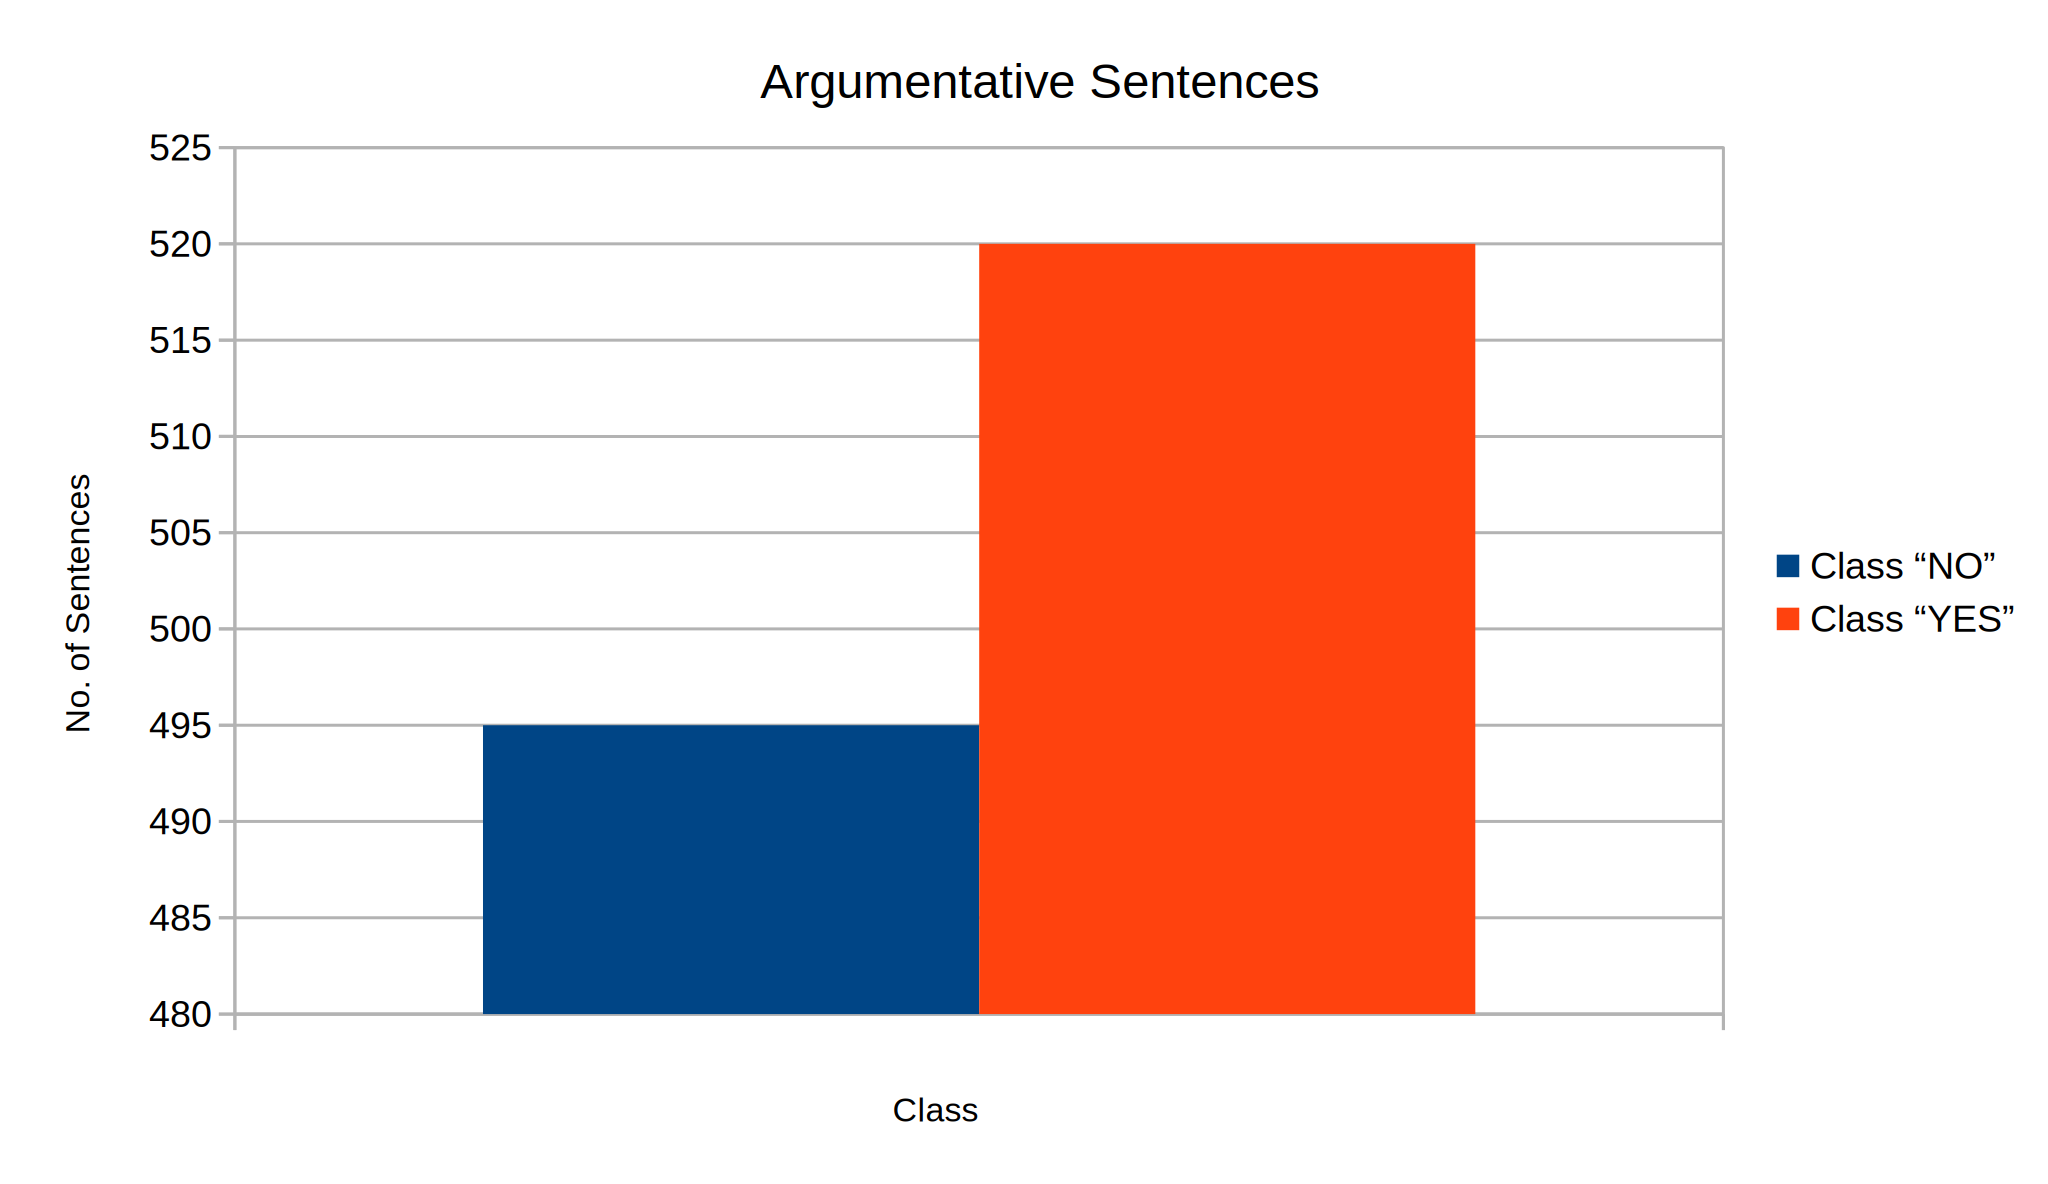
\includegraphics[width=0.9\linewidth]{figure/arguments/A_argumentative1.pdf}
\caption{Argumentative Sentences in Train Set.}
\end{figure}

\begin{figure}[H]
\centering
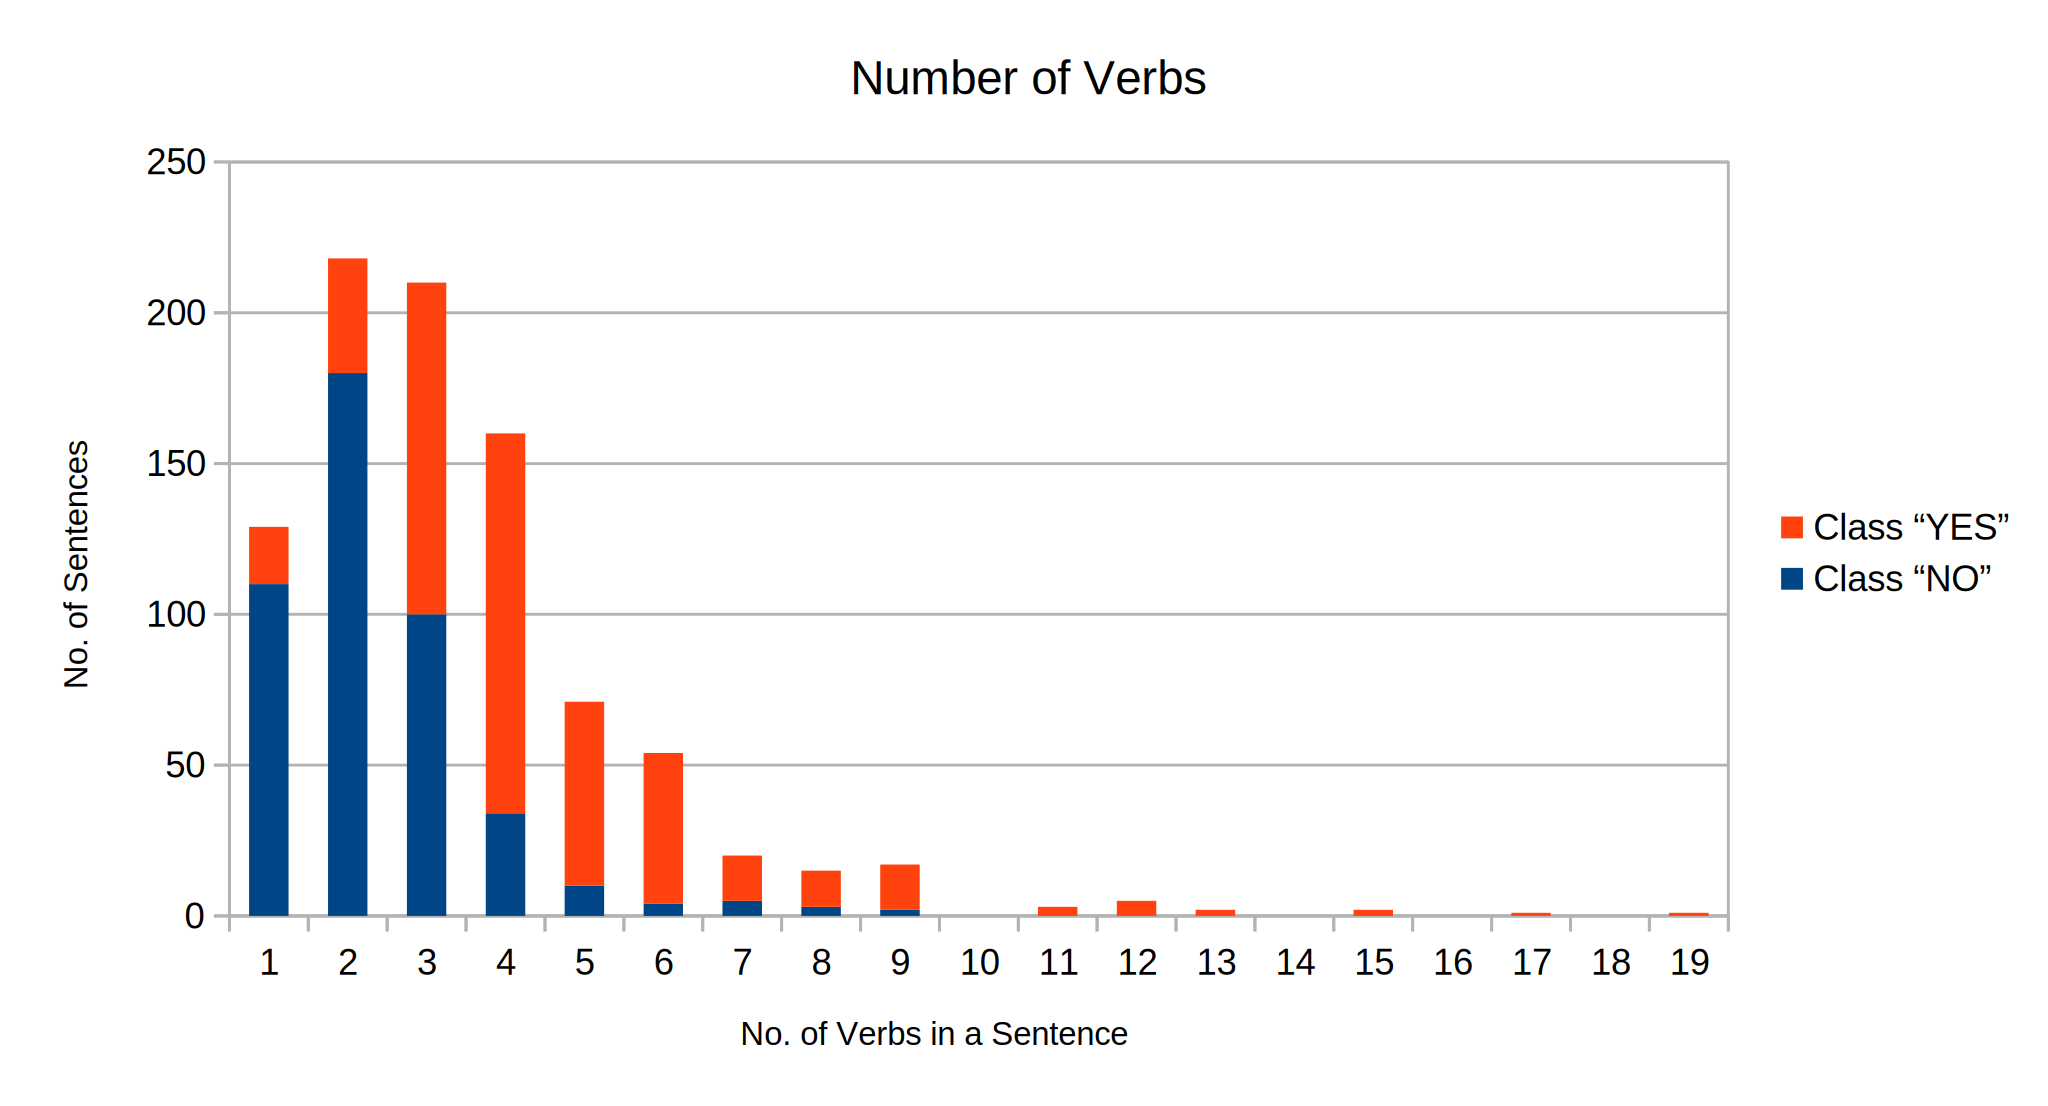
\includegraphics[width=0.8\linewidth]{figure/arguments/A_verbs1.pdf}
\caption{Argument Marker - Number of Verbs}
\end{figure}

\begin{figure}[H]
\centering
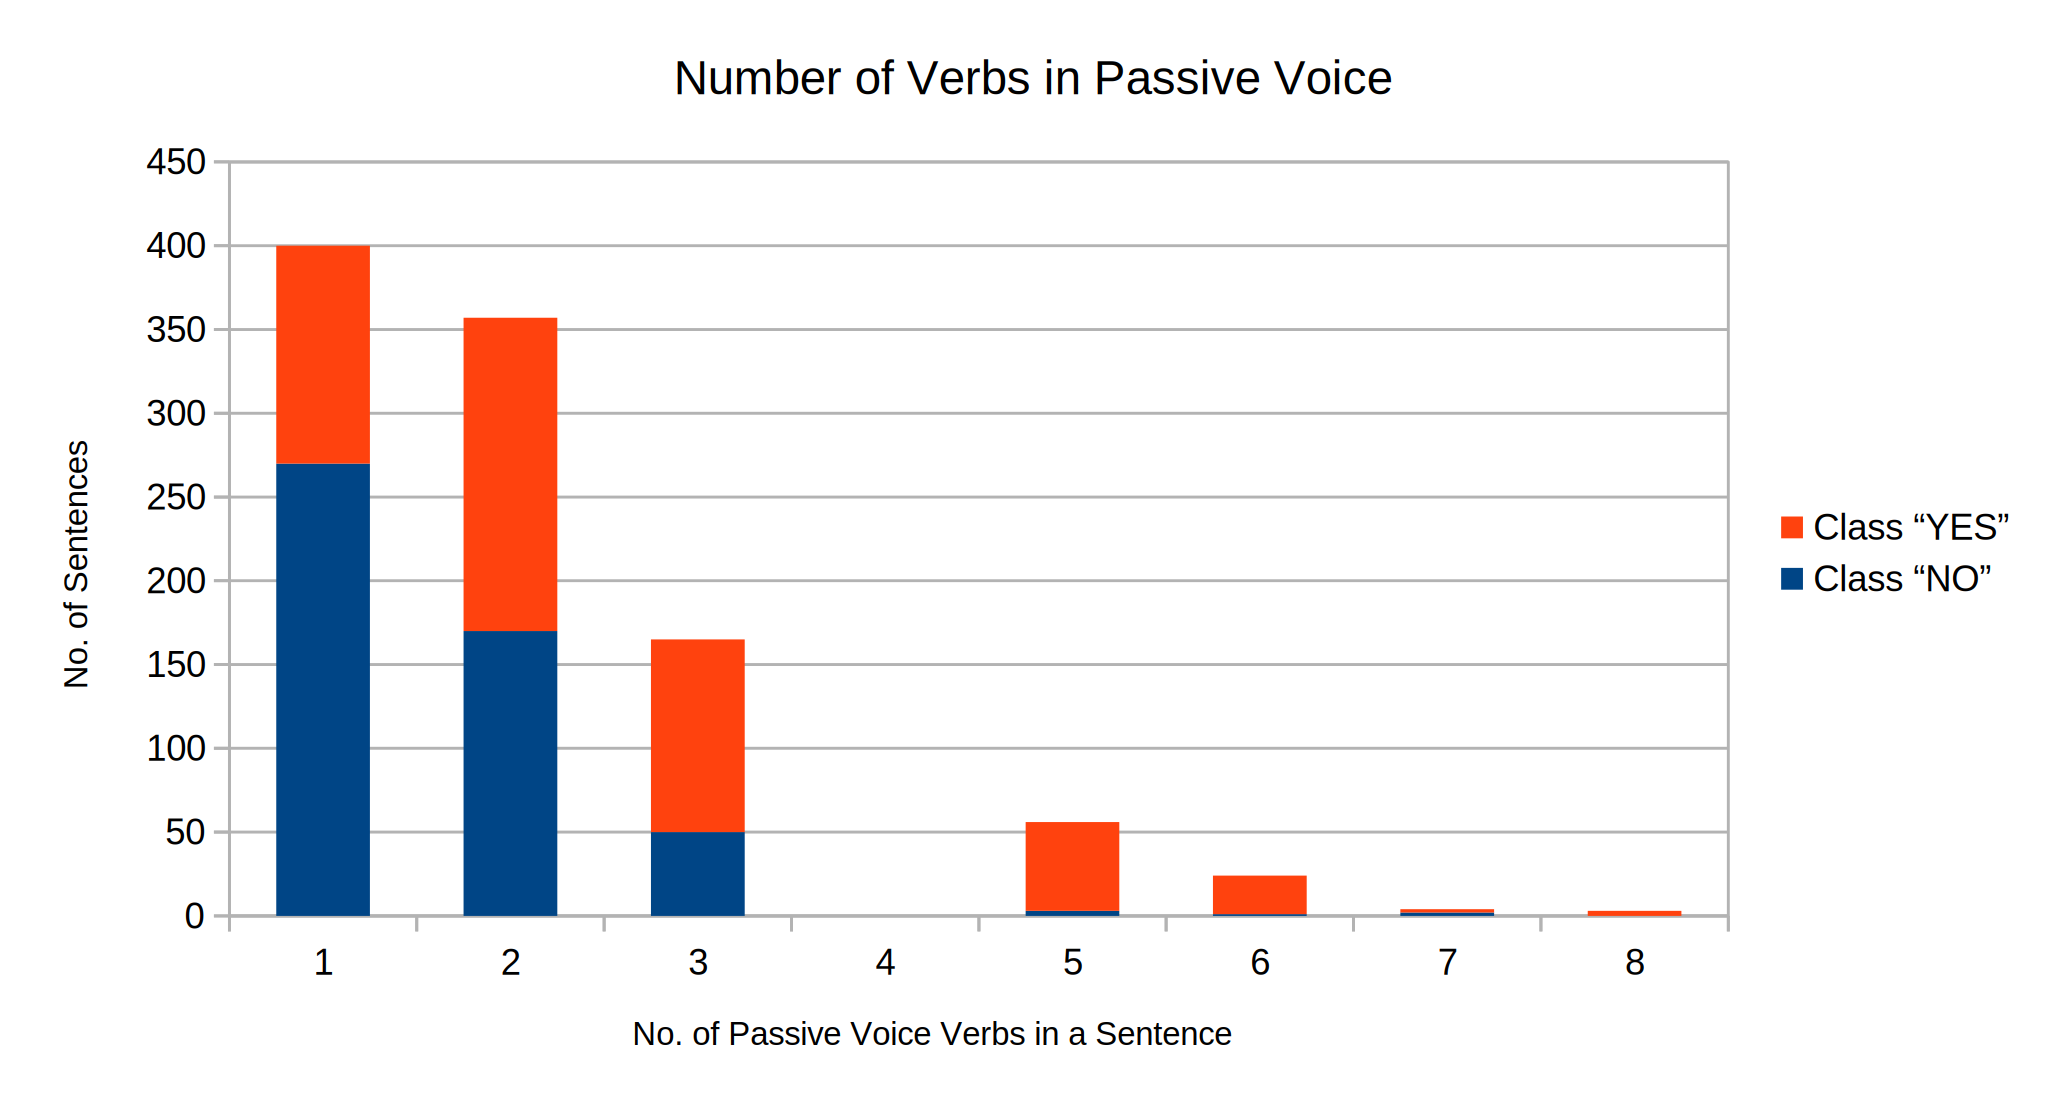
\includegraphics[width=0.8\linewidth]{figure/arguments/A_pv_verbs1.pdf}
\caption{Argument Marker - Number of Verbs in Passive Voice}
\end{figure}

\begin{figure}[H]
\centering
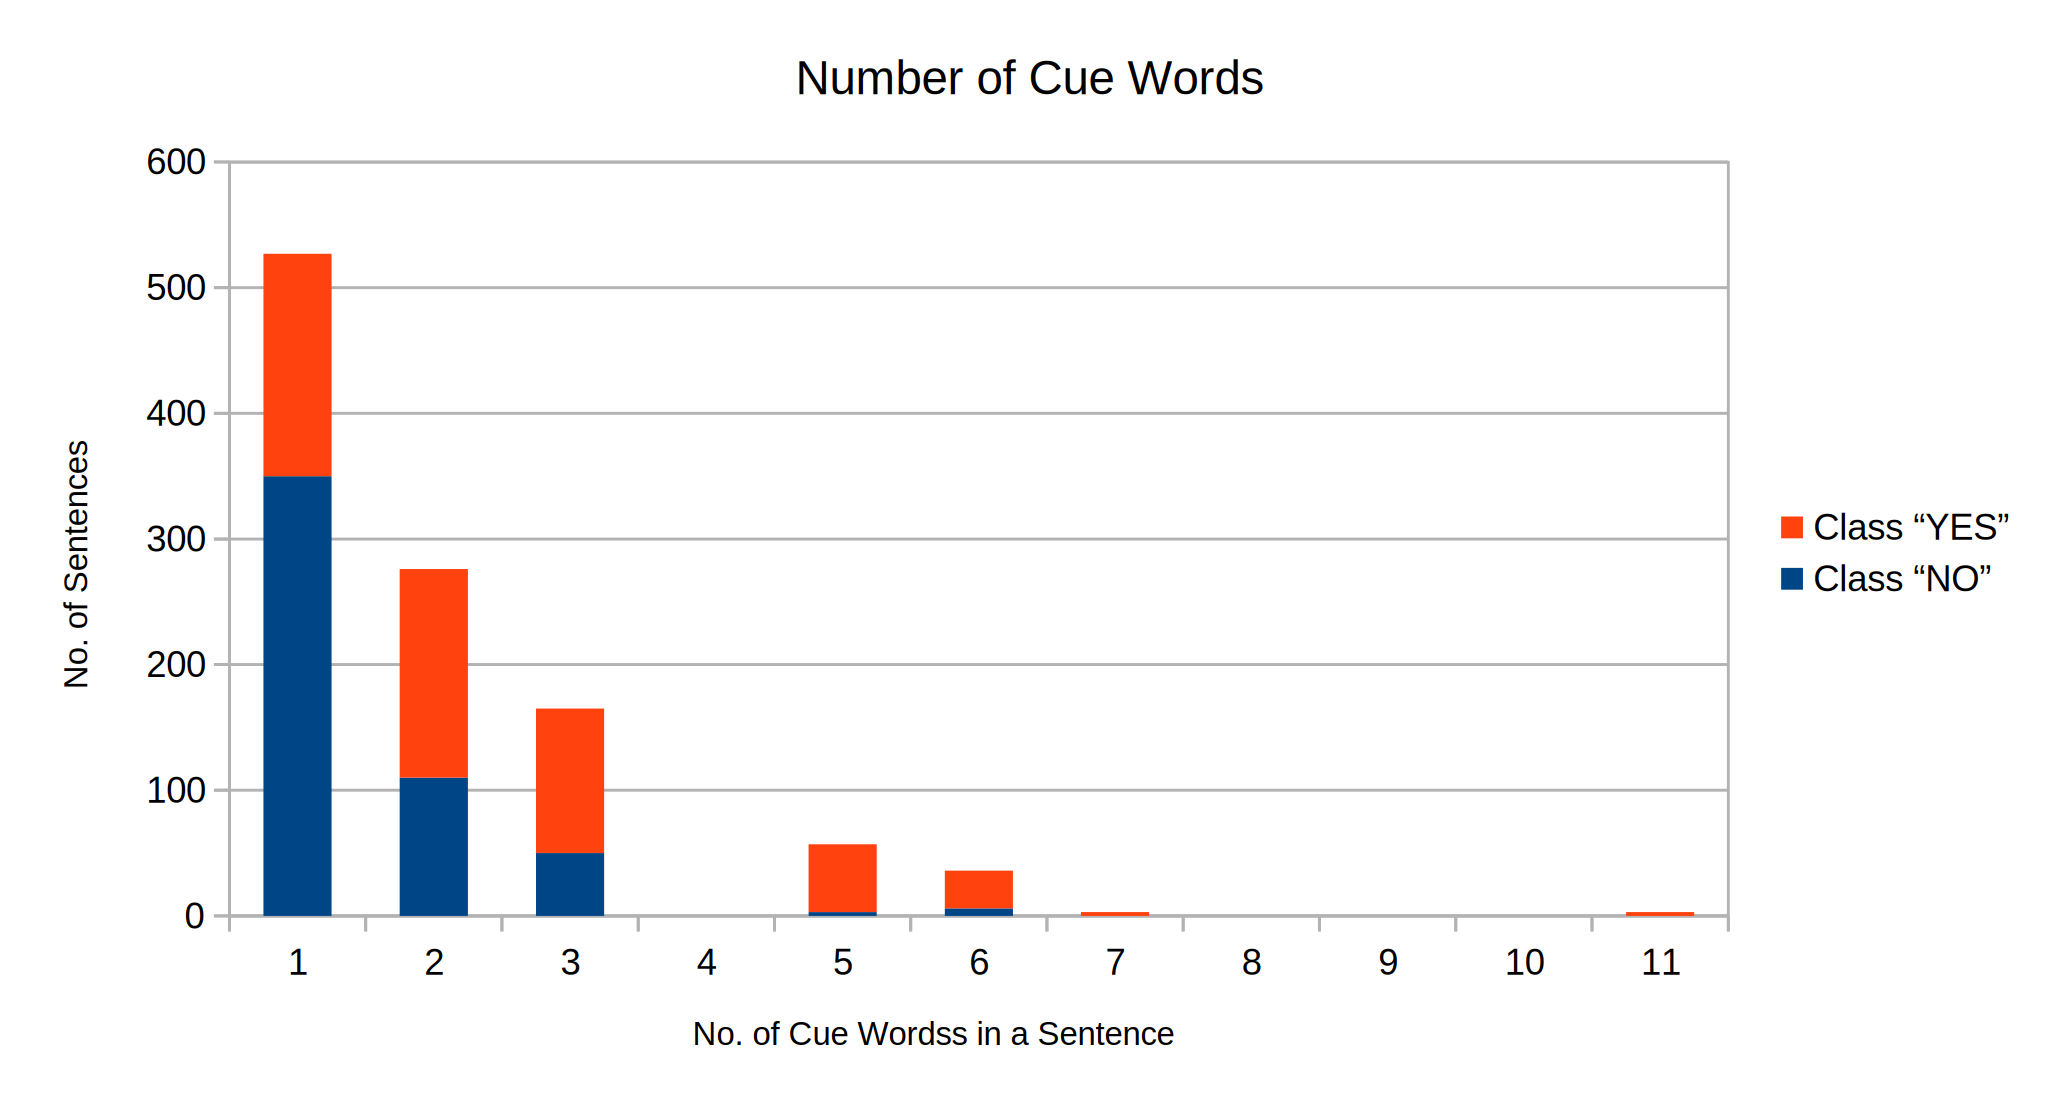
\includegraphics[width=0.8\linewidth]{figure/arguments/A_cue_words1.pdf}
\caption{Argument Marker - Number of Cue Words}
\end{figure}

\begin{figure}[H]
\centering
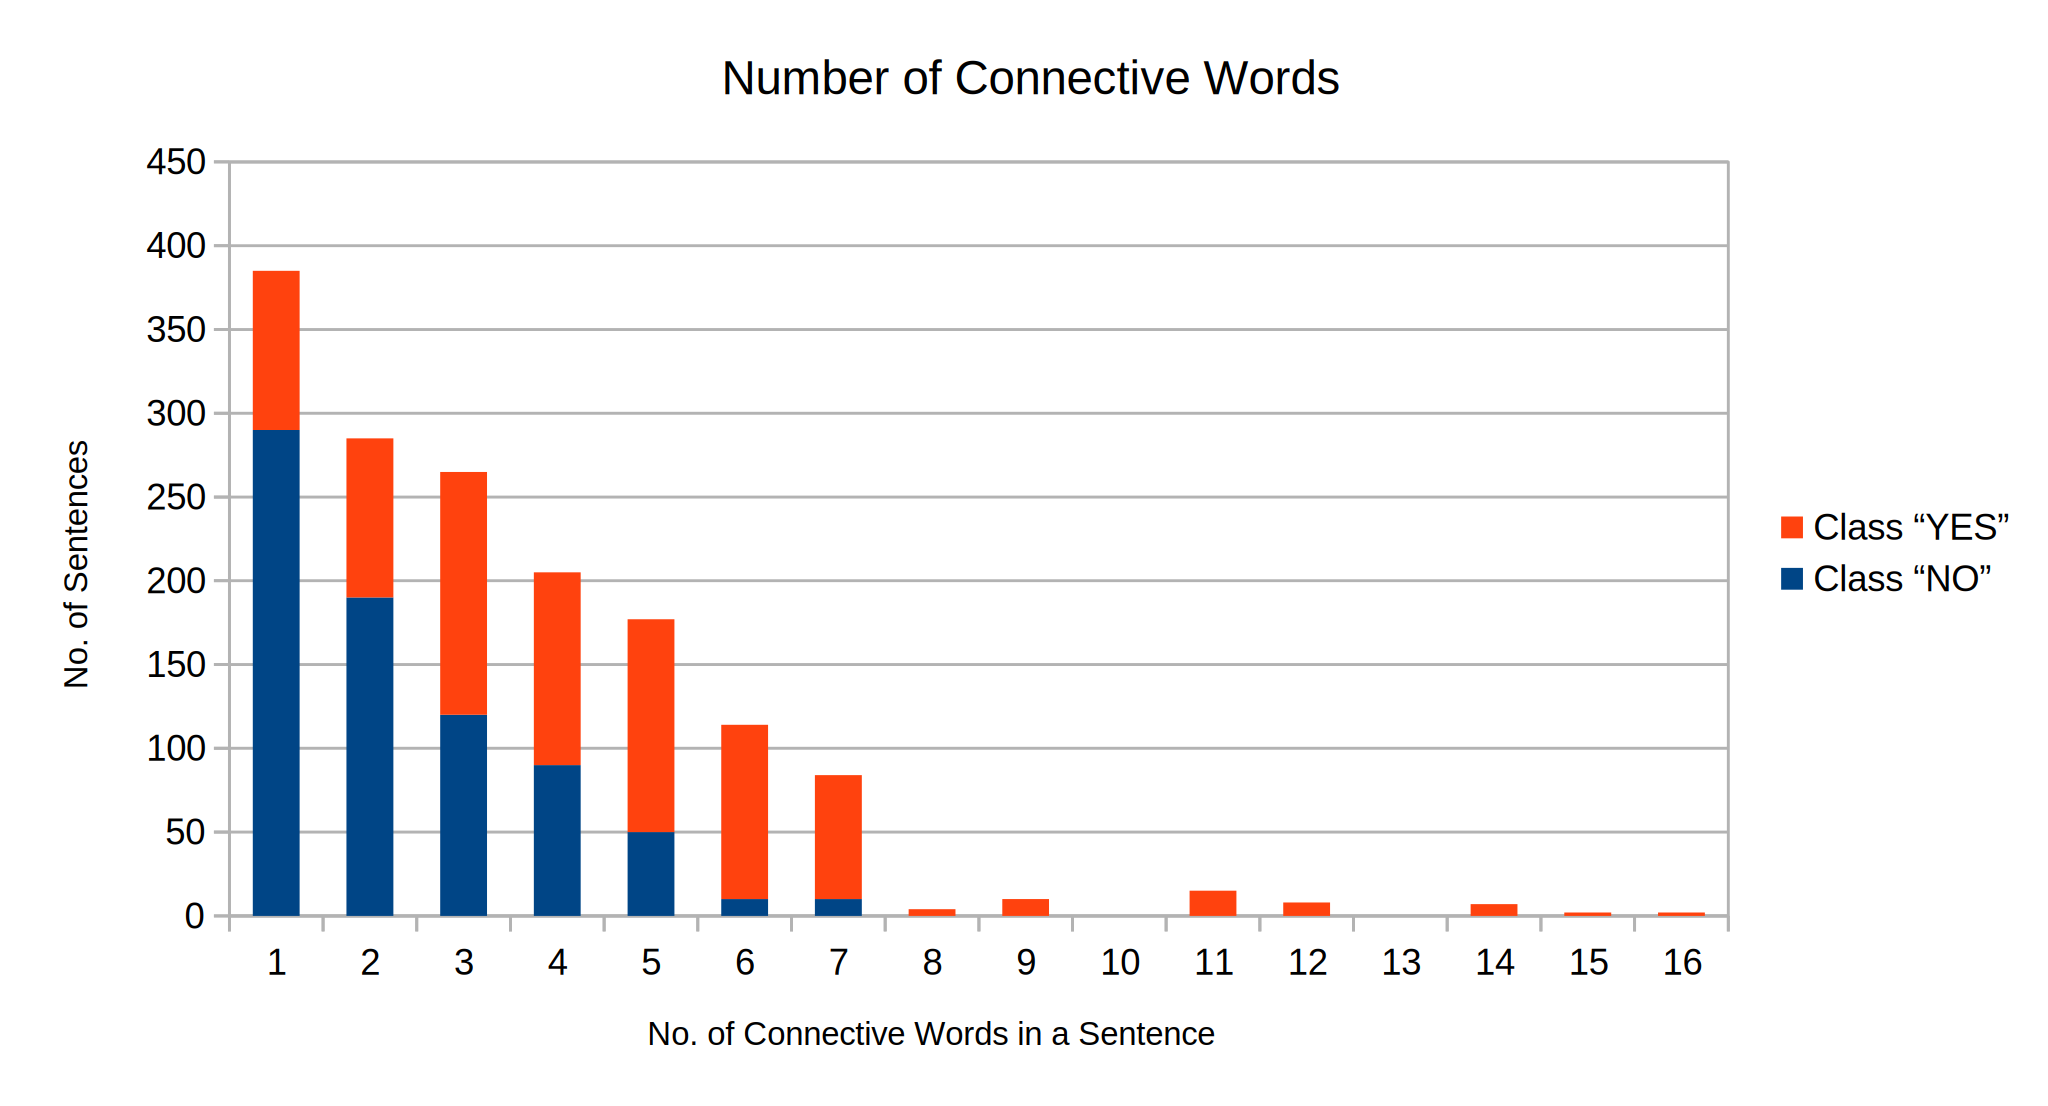
\includegraphics[width=0.8\linewidth]{figure/arguments/A_connective1.pdf}
\caption{Argument Marker - Number of Connective Words}
\end{figure}

\begin{figure}[H]
\centering
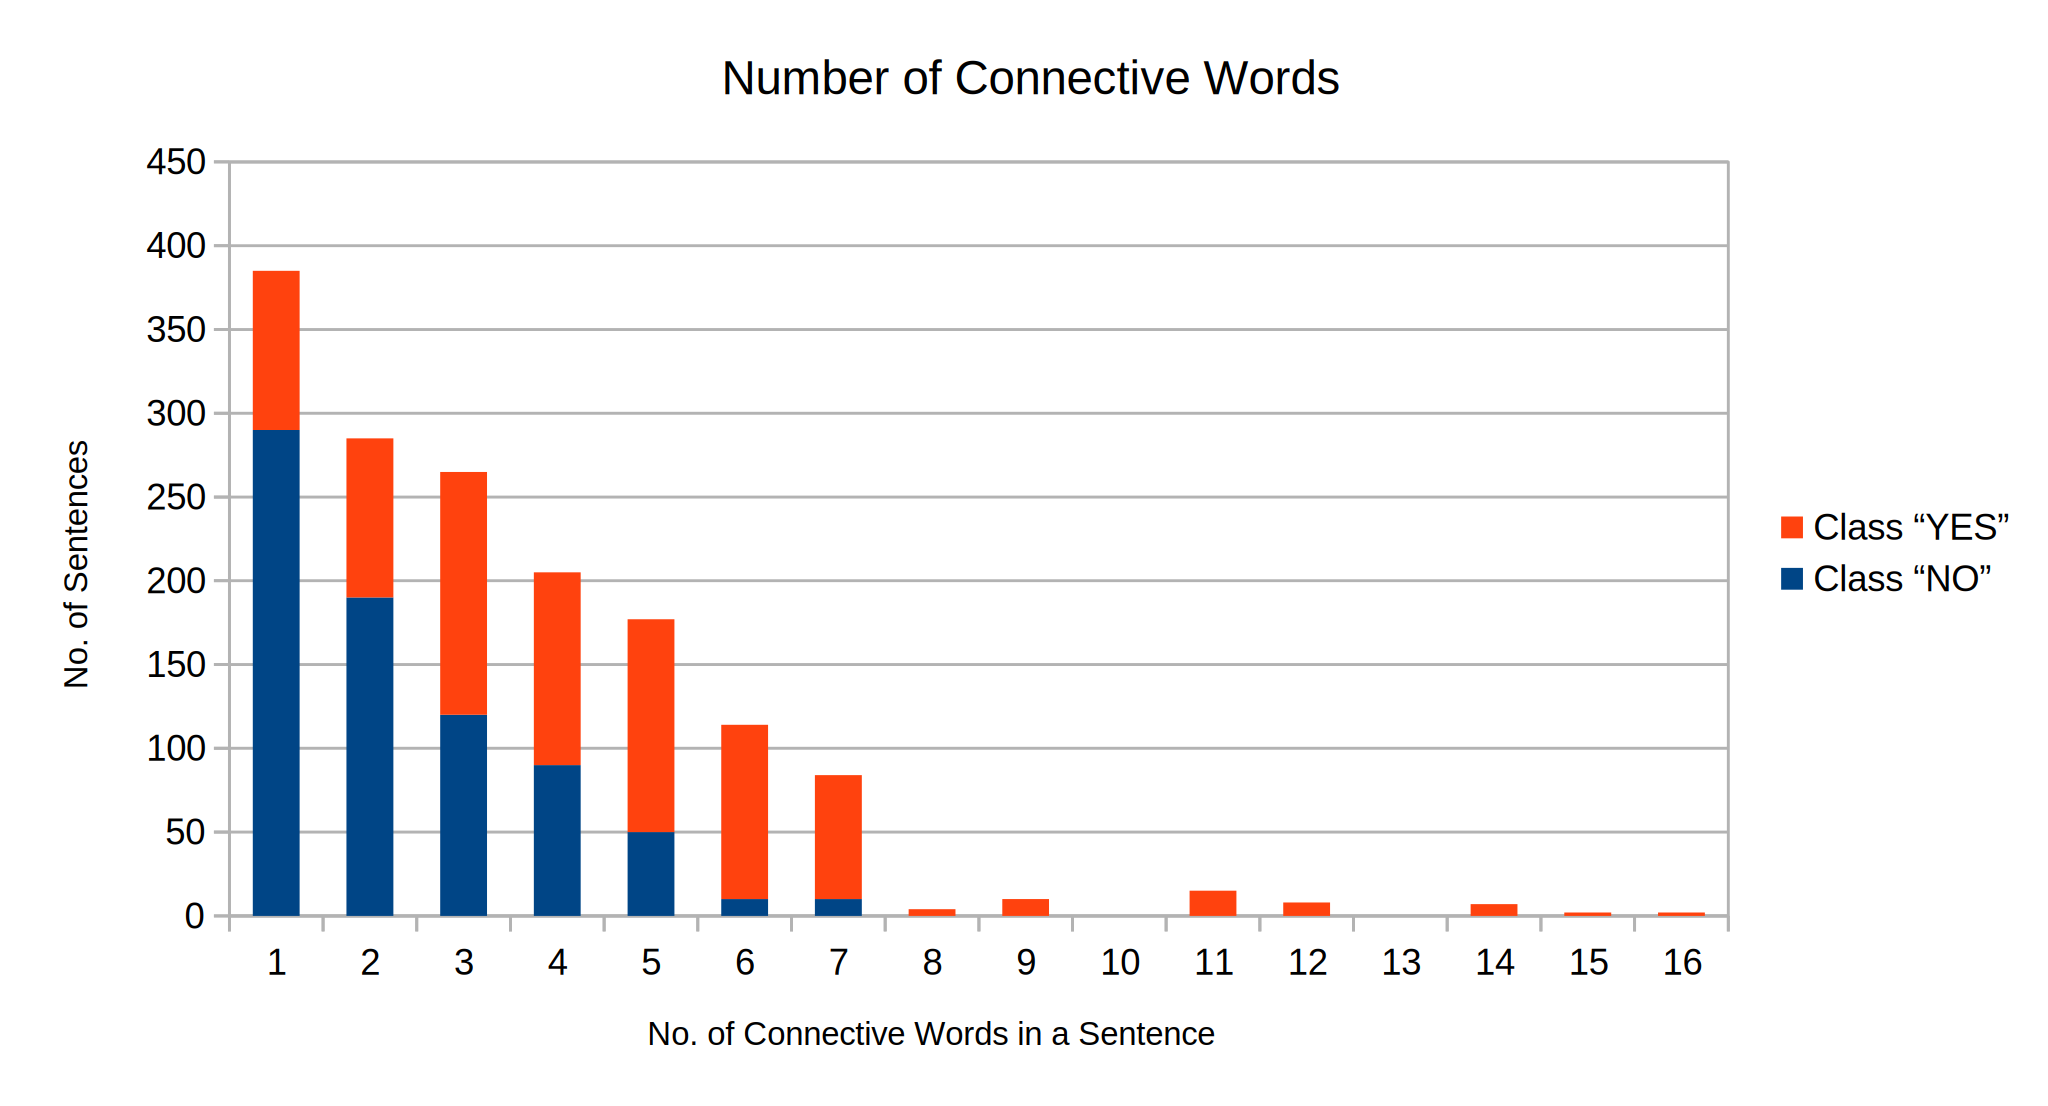
\includegraphics[width=0.8\linewidth]{figure/arguments/A_connective1.pdf}
\caption{Argumentative Sentences in Train Set.}
\end{figure}

\begin{figure}[H]
\centering
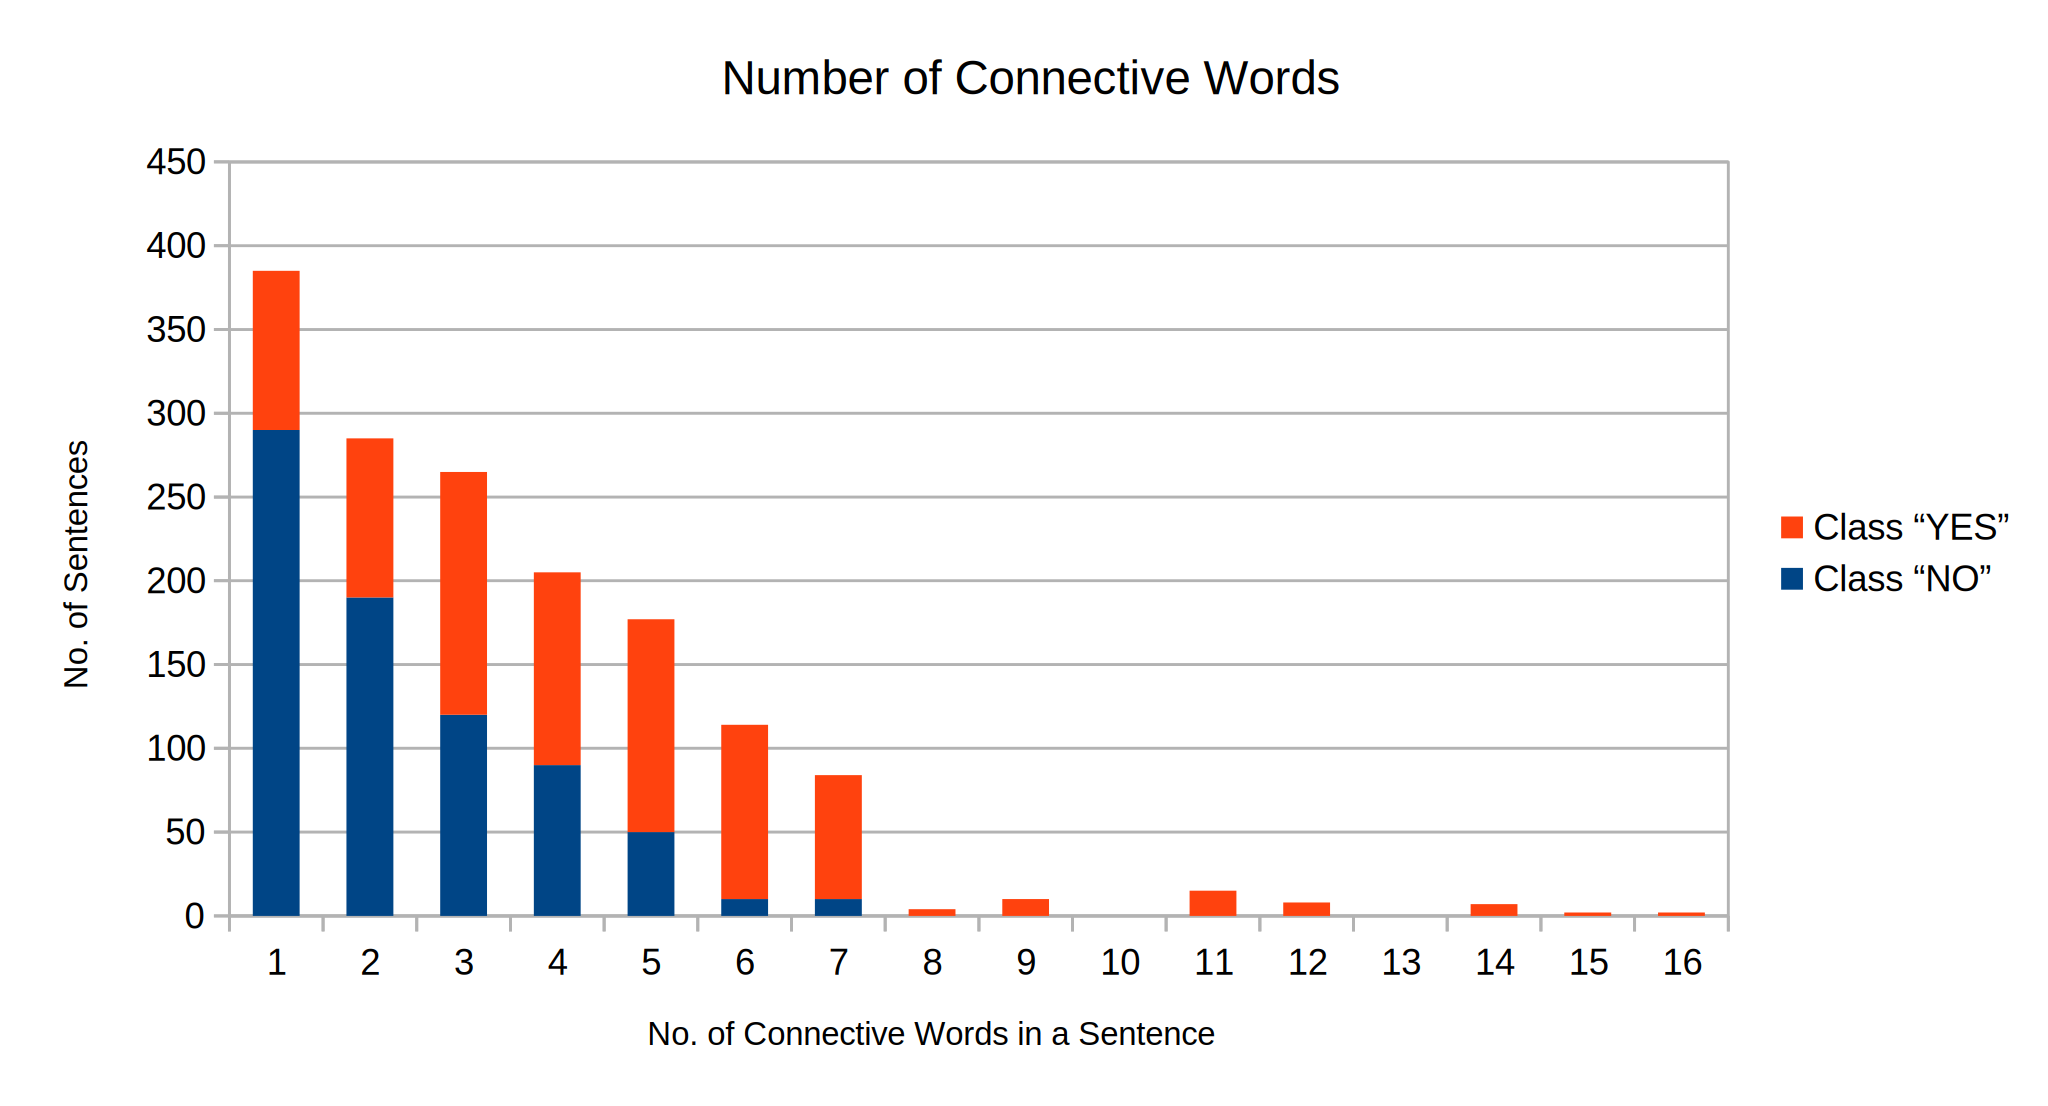
\includegraphics[width=0.8\linewidth]{figure/arguments/A_connective1.pdf}
\caption{Argumentative Sentences in Train Set.}
\end{figure}

\begin{figure}[H]
\centering
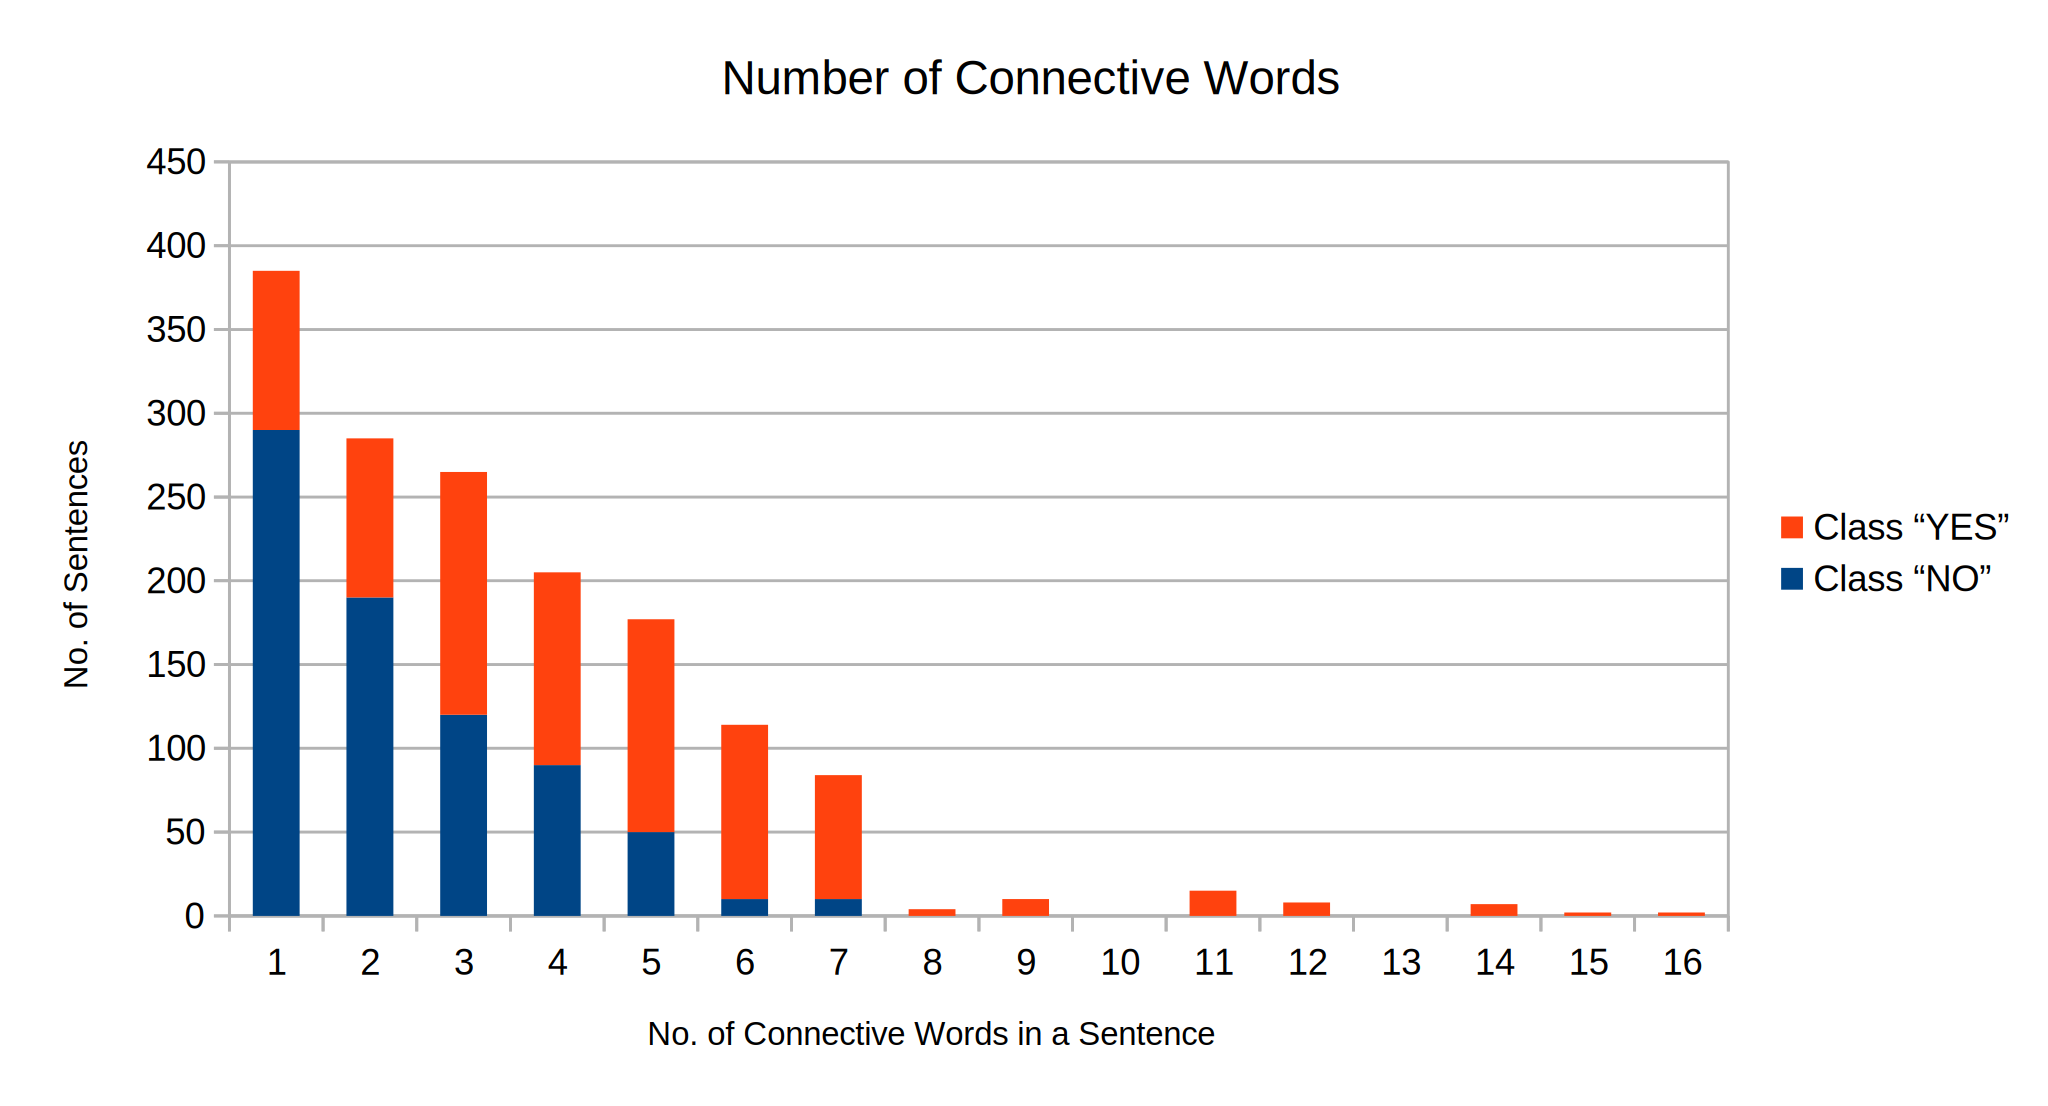
\includegraphics[width=0.8\linewidth]{figure/arguments/A_connective1.pdf}
\caption{Argumentative Sentences in Train Set.}
\end{figure}

\begin{figure}[H]
\centering
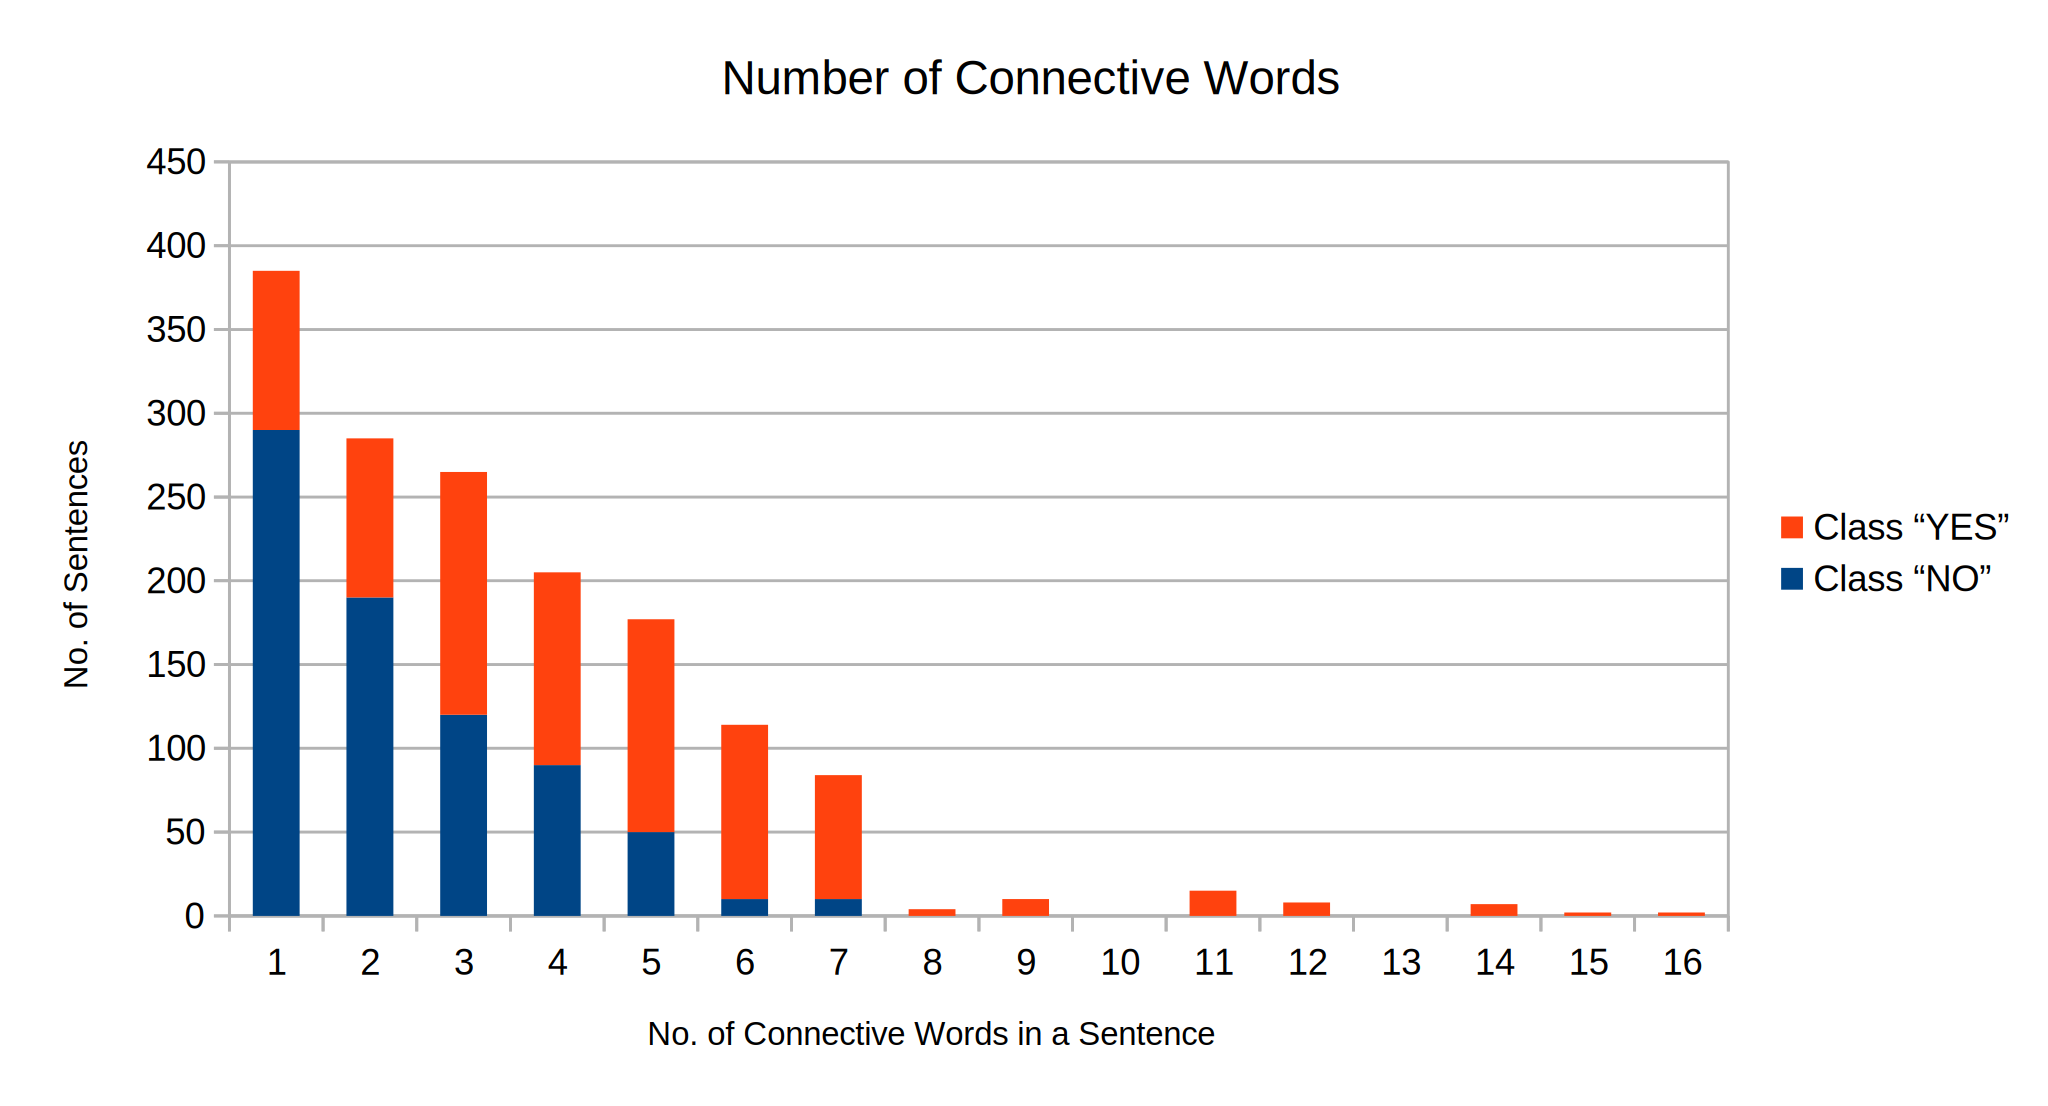
\includegraphics[width=0.8\linewidth]{figure/arguments/A_connective1.pdf}
\caption{Argumentative Sentences in Train Set.}
\end{figure}

\begin{figure}[H]
\centering
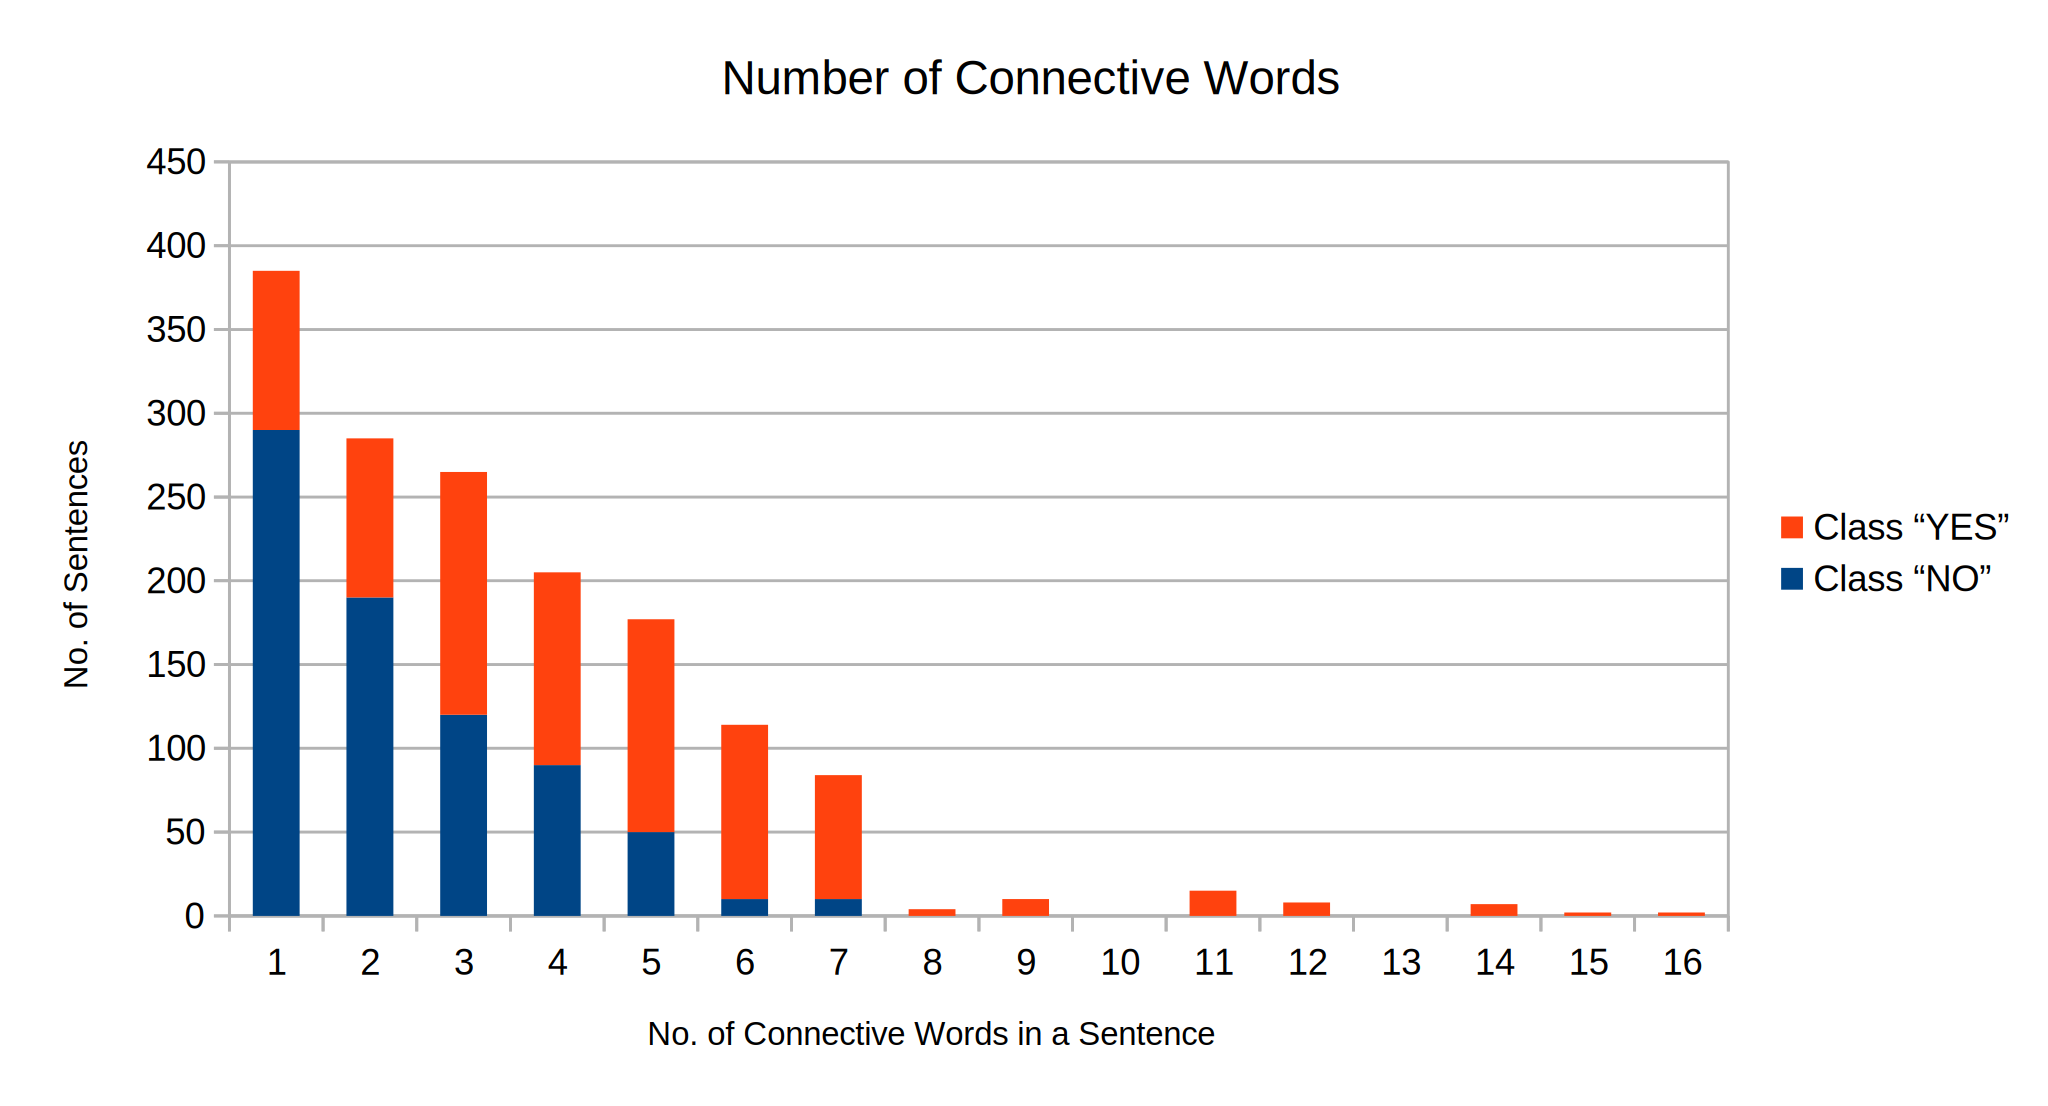
\includegraphics[width=0.8\linewidth]{figure/arguments/A_connective1.pdf}
\caption{Argumentative Sentences in Train Set.}
\end{figure}

\subsection{Algorithms used in Machine Learning Procedure}\label{412_ref}
TODO\\
\\

\begin{table}[H]
\centering
\caption{Detailed Accuracy for Class “No” (Argument Extraction).}
\label{41_table_ref}
\begin{tabular}{cccc}
\hline
{\bf Algorithm}     & {\bf Precision} & {\bf Recall}    & {\bf F-Measure} \\ \hline
SVM                 & {\it 0.815}     & {\it 0.830}     & {\bf 0.823} \\
Random Forest       & {\bf 0.818} 	 & {\it 0.818}     & {\it 0.818}     \\
Native Bayes        & {\it 0.718}     & {\bf 0.899}     & {\it 0.798}     \\
Logistic Regression & {\it 0.801}     & {\it 0.819}     & {\it 0.819}     \\ \hline
\end{tabular}
\end{table}

\begin{table}[H]
\centering
\caption{Detailed Accuracy for Class “Yes” (Argument Extraction).}
\label{42_table_ref}
\begin{tabular}{cccc}
\hline
{\bf Algorithm}     & {\bf Precision} & {\bf Recall}    & {\bf F-Measure} \\ \hline
SVM                 & {\it 0.836}     & {\it 0.821}     & {\bf 0.828} \\
Random Forest       & {\it 0.827}     & {\bf 0.827}	   & {\it 0.827}     \\
Native Bayes        & {\bf 0.873} 	 & {\it 0.663}     & {\it 0.754}     \\
Logistic Regression & {\it 0.837}     & {\it 0.802}     & {\it 0.819}     \\ \hline
\end{tabular}
\end{table}

\begin{table}[H]
\centering
\caption{Weighted Average on both Classes (Argument Extraction).}
\label{43_table_ref}
\begin{tabular}{cccc}
\hline
{\bf Algorithm}     & {\bf Precision} & {\bf Recall}    & {\bf F-Measure} \\ \hline
SVM                 & {\bf 0.826} 	 & {\bf 0.826}     & {\bf 0.826} \\
Random Forest       & {\it 0.823}     & {\it 0.823}     & {\it 0.823}     \\
Native Bayes        & {\it 0.797}     & {\it 0.778}     & {\it 0.776}     \\
Logistic Regression & {\it 0.820}     & {\it 0.819}     & {\it 0.819}     \\ \hline
\end{tabular}
\end{table}

TODO\\
\\

\begin{table}[H]
\centering
\caption{Additional Statistical Information (Argument Extraction).}
\label{44_table_ref}
\begin{tabular}{lll}
\hline
                                   & {\bf Frequenncy} & {\bf Percentage} \\ \hline
Correctly Classified Instances     & {\it 838}        & {\it 82.56\%}    \\
Incorrectly Classified Instances   & {\it 177}        & {\it 17.4383}    \\
Kappa statistic                    & {\it 0.6512}     & {\it -}          \\
Mean absolute error                & {\it 0.1744}     & {\it -}          \\
Root mean squared error            & {\it 0.4176}     & {\it -}          \\
Relative absolute error            & {\it -}          & {\it 34.90\%}    \\
Root relative squared error        & {\it -}          & {\it 83.54\%}    \\
Coverage of cases (0.95 level)     & {\it -}          & {\it 82.56\%}    \\
Mean rel. region size (0.95 level) & {\it -}          & {\it 50\%}       \\
Total Number of Instances          & {\it 1015}       & {\it -}          \\ \hline
\end{tabular}
\end{table}


\subsection{Information about the Train Set}\label{413_ref}
TODO\\
\\

\begin{figure}[H]
\centering
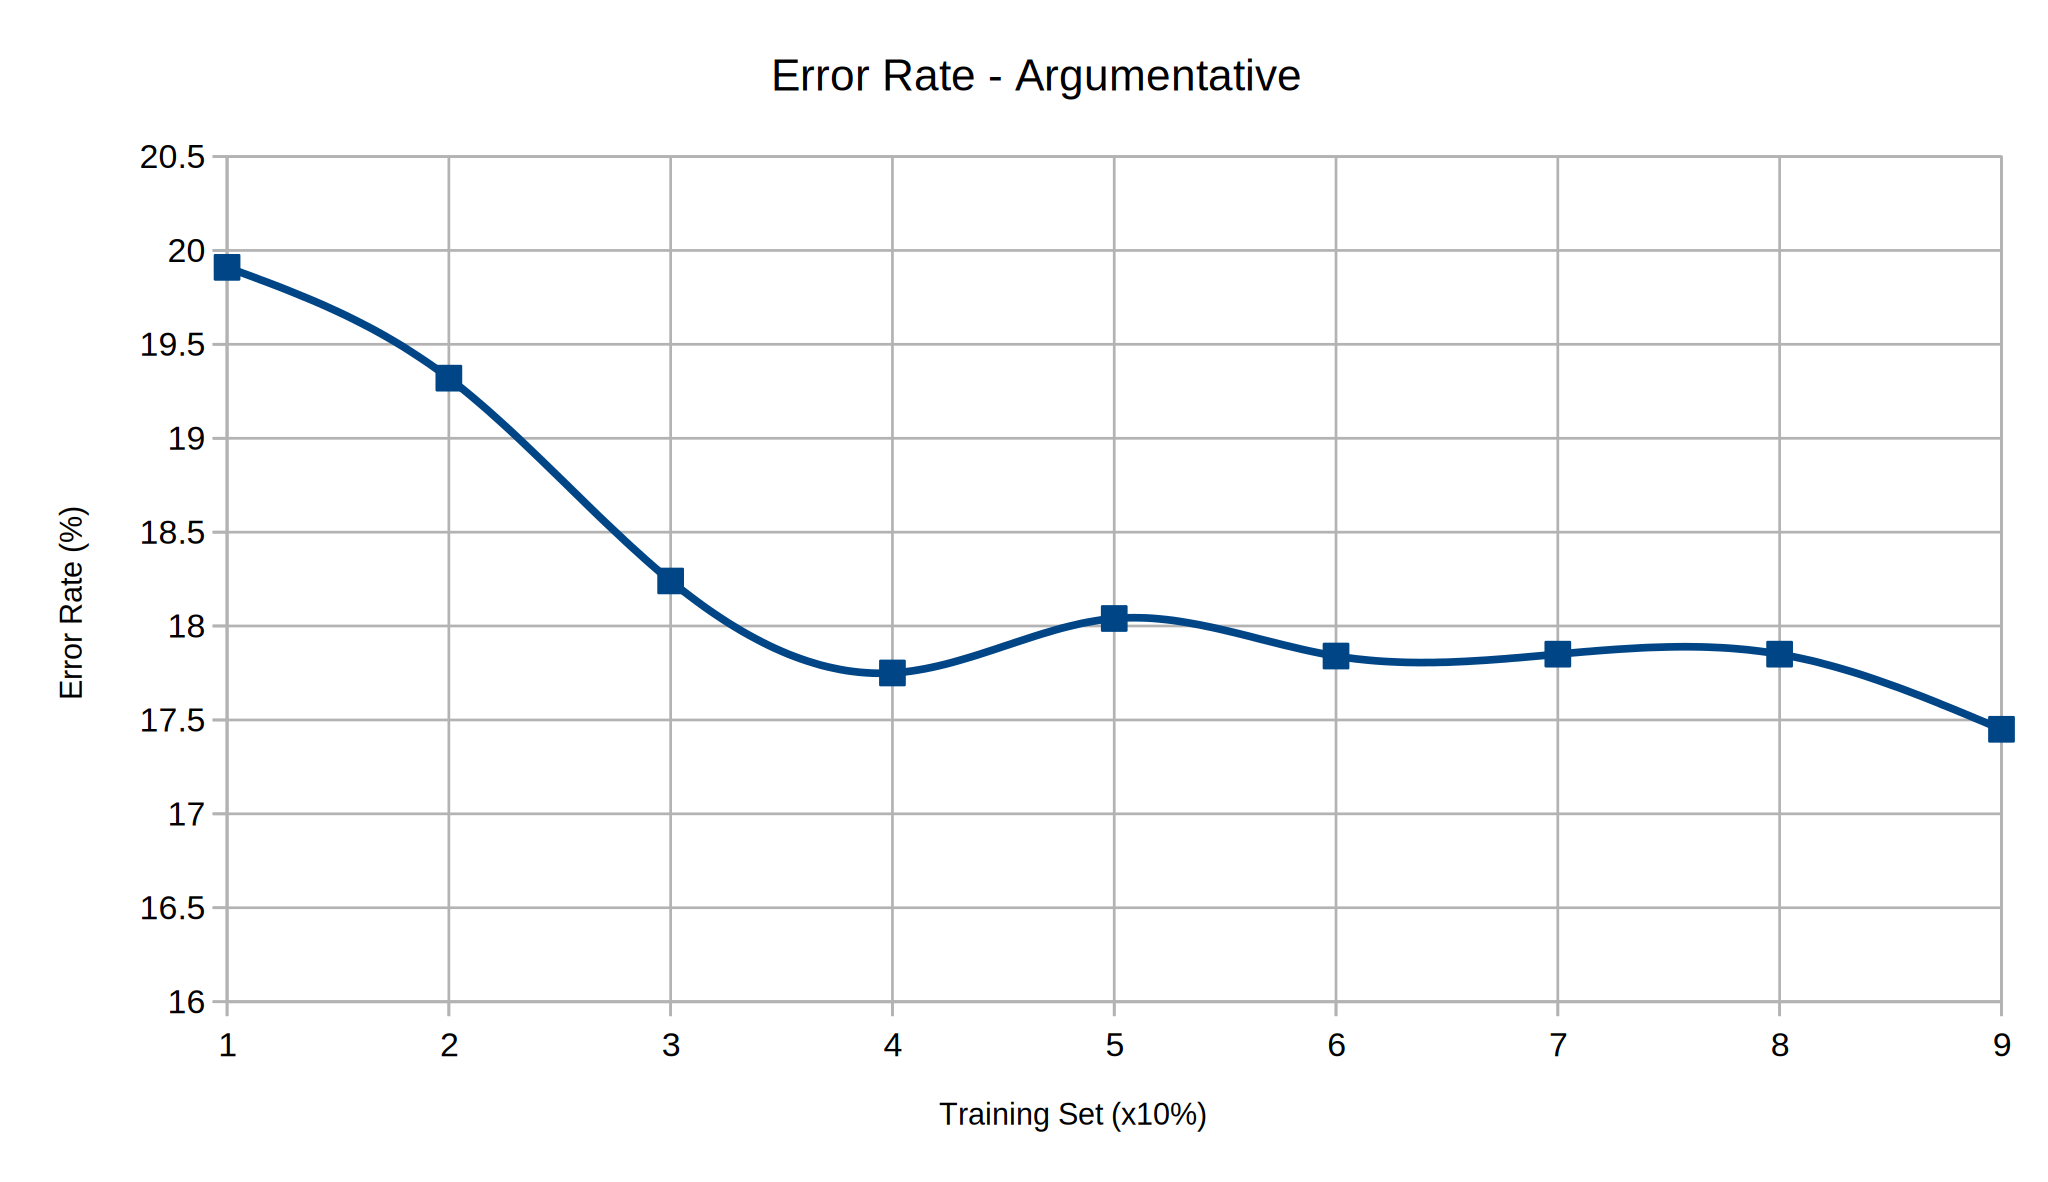
\includegraphics[width=1\linewidth]{figure/arguments/errorRate-argumentative}
\caption{Error Rate of Argumentative Sentence Classification.}
\end{figure}

\section{Suggestion Extraction}\label{42_ref}
TODO\\
\\
\subsection{``10 Fold Cross Validation'' on Train Set}\label{421_ref}
TODO\\
\\

\begin{table}[H]
\centering
\caption{Detailed Accuracy for Class “No” (Suggestion Extraction).}
\label{45_table_ref}
\begin{tabular}{cccc}
\hline
{\bf Algorithm} & {\bf Precision} & {\bf Recall} & {\bf F-Measure} \\ \hline
J48             & {\it 0.881}     & {\it 0.923}  & {\it 0.901}     \\
Random Forest   & {\it 0.890}      & {\it 0.915}  & {\it 0.902}     \\
Native Bayes    & {\bf 0.912}     & {\it 0.915}  & {\it 0.604}     \\
SVM             & {\it 0.839}     & {\bf 0.989}  & {\bf 0.908}     \\ \hline
\end{tabular}
\end{table}

\begin{table}[H]
\centering
\caption{Detailed Accuracy for Class “Yes” (Suggestion Extraction).}
\label{46_table_ref}
\begin{tabular}{cccc}
\hline
{\bf Algorithm} & {\bf Precision} & {\bf Recall} & {\bf F-Measure} \\ \hline
J48             & {\it 0.552}     & {\it 0.432}  & {\it 0.485}     \\
Random Forest   & {\it 0.556}     & {\it 0.489}  & {\it 0.519}     \\
Native Bayes    & {\it 0.608}     & {\bf 0.601}  & {\bf 0.604}     \\
SVM             & {\bf 0.735}     & {\it 0.137}  & {\it 0.230}     \\ \hline
\end{tabular}
\end{table}

\begin{table}[H]
\centering
\caption{Weighted Average on both Classes (Suggestion Extraction).}
\label{47_table_ref}
\begin{tabular}{cccc}
\hline
{\bf Algorithm} & {\bf Precision} & {\bf Recall} & {\bf F-Measure} \\ \hline
J48             & {\it 0.822}     & {\it 0.834}  & {\it 0.826}     \\
Random Forest   & {\it 0.830}      & {\it 0.837}  & {\it 0.833}     \\
Native Bayes    & {\bf 0.858}     & {\bf 0.858}  & {\bf 0.858}     \\
SVM             & {\it 0.820}      & {\it 0.835}  & {\it 0.786}     \\ \hline
\end{tabular}
\end{table}

TODO\\
\\

\begin{table}[H]
\centering
\caption{Additional Statistical Information (Suggestion Extraction).}
\label{48_table_rer}
\begin{tabular}{lll}
\hline
                                   & {\bf Frequenncy} & {\bf Percentage} \\ \hline
Correctly Classified Instances     & {\it 871}        & {\it 85.81\%}    \\
Incorrectly Classified Instances   & {\it 144}        & {\it 14.19\%}    \\
Kappa statistic                    & {\it 0.518}      & {\it -}          \\
Mean absolute error                & {\it 0.1901}     & {\it -}          \\
Root mean squared error            & {\it 0.3382}     & {\it -}          \\
Relative absolute error            & {\it -}          & {\it 64.21\%}    \\
Root relative squared error        & {\it -}          & {\it 87.98\%}    \\
Coverage of cases (0.95 level)     & {\it -}          & {\it 95.67\%}    \\
Mean rel. region size (0.95 level) & {\it -}          & {\it 70.64\%}    \\
Total Number of Instances          & {\it 1015}       & {\it -}          \\ \hline
\end{tabular}
\end{table}


\subsection{Equivalent Train Set}\label{422_ref}
TODO\\
\\

\begin{table}[H]
\centering
\caption{Detailed Accuracy for Class “No” (Suggestion Extraction, using Equivalent Train Set).}
\label{49_table_rer}
\begin{tabular}{cccc}
\hline
{\bf Algorithm} & {\bf Precision} & {\bf Recall} & {\bf F-Measure} \\ \hline
J48             & {\it 0.940}      & {\it 0.810}   & {\it 0.870}      \\
Random Forest   & {\bf 0.996}     & {\it 0.810}   & {\bf 0.893}     \\
Native Bayes    & {\it 0.941}     & {\bf 0.828}  & {\it 0.881}     \\
SVM             & {\it 0.939}     & {\it 0.819}  & {\it 0.875}     \\ \hline
\end{tabular}
\end{table}

\begin{table}[H]
\centering
\caption{Detailed Accuracy for Class “Yes” (Suggestion Extraction, using Equivalent Train Set).}
\label{410_table_rer}
\begin{tabular}{cccc}
\hline
{\bf Algorithm} & {\bf Precision} & {\bf Recall} & {\bf F-Measure} \\ \hline
J48             & {\it 0.470}      & {\it 0.765}  & {\it 0.582}     \\
Random Forest   & {\bf 0.533}     & {\bf 0.984}  & {\bf 0.641}     \\
Native Bayes    & {\it 0.495}     & {\it 0.765}  & {\it 0.601}     \\
SVM             & {\it 0.479}     & {\it 0.760}   & {\it 0.588}     \\ \hline
\end{tabular}
\end{table}

\begin{table}[H]
\centering
\caption{Weighted Average on both Classes (Suggestion Extraction, using Equivalent Train Set).}
\label{411_table_rer}
\begin{tabular}{cccc}
\hline
{\bf Algorithm} & {\bf Precision} & {\bf Recall} & {\bf F-Measure} \\ \hline
J48             & {\it 0.855}     & {\it 0.802}  & {\it 0.818}     \\
Random Forest   & {\bf 0.912}     & {\bf 0.841}  & {\bf 0.857}     \\
Native Bayes    & {\it 0.861}     & {\it 0.817}  & {\it 0.831}     \\
SVM             & {\it 0.856}     & {\it 0.808}  & {\it 0.823}     \\ \hline
\end{tabular}
\end{table}

TODO\\
\\

\begin{table}[H]
\centering
\caption{Additional Statistical Information (Suggestion Extraction, using Equivalent Train Set).}
\label{412_table_rer}
\begin{tabular}{ccc}
\hline
                                   & {\bf Frequenncy} & {\bf Percentage} \\ \hline
Correctly Classified Instances     & {\it 854}        & {\it 84.14\%}    \\
Incorrectly Classified Instances   & {\it 161}        & {\it 15.86\%}    \\
Kappa statistic                    & {\it 0.5966}     & {\it -}          \\
Mean absolute error                & {\it 0.2273}     & {\it -}          \\
Root mean squared error            & {\it 0.3467}     & {\it -}          \\
Relative absolute error            & {\it -}          & {\it 47.98\%}    \\
Root relative squared error        & {\it -}          & {\it 73.02\%}    \\
Coverage of cases (0.95 level)     & {\it -}          & {\it 97.14\%}    \\
Mean rel. region size (0.95 level) & {\it -}          & {\it 83.00\%}    \\
Total Number of Instances          & {\it 1015}       & {\it -}          \\ \hline
\end{tabular}
\end{table}


\section{Overall Opinion Extraction}\label{43_ref}
TODO\\
\\

